%Template pembuatan proposal skripsi.
\documentclass{jtetiproposalskripsi}

%-----------------------------------------------------------------
%Disini awal masukan untuk data proposal skripsi
%-----------------------------------------------------------------
\titleind{ANALISA PERFORMA PENGOLAH PARALEL 
BERBASIS KLASTER DAN NON KLASTER}

\fullname{RISKI RAHMAD TULLAH}

\idnum{1110651099}

\approvaldate{}

\degree{Sarjana Komputer}

\yearsubmit{2015}

\program{Teknik Informatika}

\headprogram{Agung Nilogiri, S.Kom M.Kom.}

\dept{Teknik Informatika}

\firstsupervisor{Triawan Adi Cahyanto, M.Kom}
\firstnip{}

\secondsupervisor{}
\secondnip{}


%-----------------------------------------------------------------
%Disini akhir masukan untuk data proposal skripsi
%-----------------------------------------------------------------

\begin{document}

\cover

\approvalpage

%-----------------------------------------------------------------
%Disini akhir masukan untuk muka skripsi
%-----------------------------------------------------------------

%-----------------------------------------------------------------
%Disini awal masukan Intisari
%-----------------------------------------------------------------
\begin{abstractind}
Klaster komputer pribadi atau personal computer adalah kumpulan Komputer yang terhubungkan dalam sebuah jaringan komputer dan berfungsi sebagai sebuah komputer untuk menyelesaikan suatu persoalan secara bersamaan \emph{Simultaneous}, Dengan menggunakan klaster komputer ini diharapkan suatu program atau persoalan dapat dieksekusi dengan lebih cepat dibandingakan tanpa mengunakan metode klaster. Namun hanya problem yang dapat dipilah menjadi beberapa bagian dan dapat diproses secara terpisahlah yang dapat memanfaatkan teknik klaster ini secara maksimal. Baik dalam segi kecepatan proses penyelesaian serta akurasi. Oleh karna itu penelitian ini akan membahas tentang \emph{Analisa Performa Pengolah Paralel Berbasis Klaster Dan Non Klater}. Untuk mengetahui perbedaan kecepatan dari penyelesaian sebuah proses yang sedang dilakukan .


\bigskip
\textbf{Kata kunci} : \emph{Analisa Performa}, \emph{paralel}, Non paralel.
\end{abstractind}
%-----------------------------------------------------------------
%Disini akhir masukan Intisari
%-----------------------------------------------------------------

\tableofcontents
\addcontentsline{toc}{chapter}{DAFTAR ISI}
\selectlanguage{bahasa}\clearpage\pagenumbering{arabic}\setcounter{page}{1}

%-----------------------------------------------------------------
%Disini awal masukan untuk Bab
%-----------------------------------------------------------------
\chapter{LATAR BELAKANG}

\section{Latar Belakang Masalah}
Perkembangan teknologi dan ilmu pengetahuan pada masa globalisasi ini dirasakan telah semakin pesat dan canggih. Semua ini dikarenakan hasil dari pemikiran-pemikiran manusia yang semakin maju, hal  tersebut dapat dilihat dari perkembangan ilmu komputer yang semakin hari semakin berkembang dengan pesat. Selain itu perkembangan teknologi semakin mendukung bagi pengembangan hardware dan software yang mengakibatkan banyak program atau aplikasi yang tidak dapat dikerjakan oleh Komputer-komputer yang lebih dahulu muncul pada era sebelumya sehingga banyak lembaga, instansi dan orang-orang yang selalu melakukan pembaruan atau upgrade pada hardware dikarnakan tidaklagi dapat menyelesaikan problem, pekerjaan yang dihadapi serta lamanya proses yang diperlukan untuk menyelesaikan suatu pekerjaan.

Dengan adanya permasalahan yang dihadapi sebagaimana dijelaskan diatas makan dibutuhkan metode atau cara agar sumberdaya komputer yang ada tidak menjadi sia-sia serta dapat digunakan untuk menjalankan progran-program yang memerlukan sumberdaya yang cukup besar guna menyelesaikan masalah, pekerjaan atau problem yang dihadapi. Maka munculah metode \emph{Klaster} yang dapat digunakan untuk menyelesaikan masalah yang dihadapi di atas.

Untuk itu penulis mengangkat latar belakang dari permasalahan yang ada menjadi penulisan tugas yang mengambil denganjudul \emph{"analisa performa pengolah paralel Berbasis klaster dan non klaster}".


\section{Tujuan Penelitian}
Menganalisa dan membandingkan kecepatan proses antara komputer \emph{mengnunakan metode klaster dan non klaster}.

\section{Batasan Masalah}
Untuk menghindari pembahasan agar tidak menyimpang dari rumusan masalah yang ada, maka penelitian ini dibatasi yaitu  Menguji dan menganalisa performa kecepatan dari penyelesaian proses Klaster dan non Klaster agardapat digunakan untuk mengembangankan metode Klaster pada permasalahan-permasalahan berikutnya.

\section{Manfaat Penelitian}
Adapun manfaat yang diharapkan dalam penelitian iniadalah sebagai berikut : 
 
Manfaat yang dapat diambil dari penelitian ini adalah dengan adanya analisa performa paralel mengunakan Klaster dan non klaster mempermudah bagi pengembang untuk melanjutkan ke tahap penerapan konsep diatas serta dapat mengetahui perbedaan performa ataupun kecepatan pemrosessan dalam menyelesaikan persoalan sehingga mengetahui apakah metode Klaster atau non Klaster yang baik bagi pemecahan persoalan yang ada.


Selain itu, dapat memberikan wawasan tambahan bagi peneliti dan bagi orang yang membaca hasil dari penelitian ini nantinya.

%-------------------------------------------------------------------------------
\chapter{TINJAUAN PUSTAKA DAN DASAR TEORI}                

\section{Tinjauan Pustaka}
secara umum paralel komputer adalah metode yang digunakan untuk meringankan kerja komputer ketika sebuah komputer harus mangerjakan suatu program atau memecahkan masalah dalam komtek yang besar sehingga diperlukan kebutuhan spesifikasi khusus bagi komputer untuk dapat menyelesaikan permasalahan yang ada tersebut, dalam sebuah paralel komputer sebuah masalah akan di pecah menjadi beberapa bagian sehingga dengan begitu maka proses penyelesaian permasalahan dapat segera diselesaikan.

\section{Landasan Teori}
\subsection{\emph{Paralel Komputer}}
Komputasi paralel adalah salah satu teknik melakukan komputasi secara bersamaan dengan memanfaatkan beberapa komputer independen secara bersamaan. Ini umumnya diperlukan saat kapasitas yang diperlukan sangat besar, baik karena harus mengolah data dalam jumlah besar \emph{(di industri keuangan, bioinformatika, dll) }  karena tuntutan proses komputasi yang banyak. Kasus kedua umum ditemui di kalkulasi numerik untuk menyelesaikan persamaan matematis di bidang fisika \emph{(fisika komputasi)}, kimia \emph{(kimia komputasi)} dan lain-lain.

\begin{figure}
\centering
  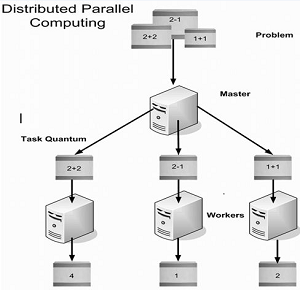
\includegraphics[height=6cm]{gambar/paralel}
\end{figure}

\begin{figure}
\centering
  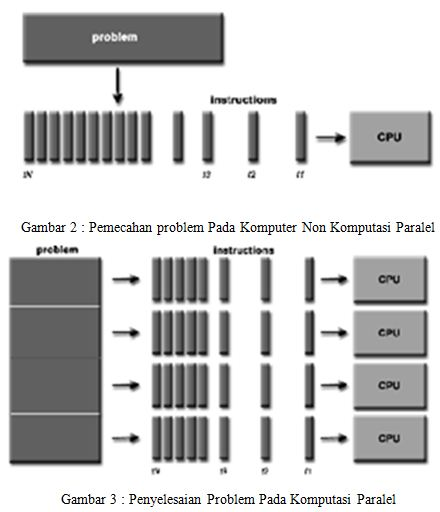
\includegraphics[height=10cm]{gambar/problem}
\end{figure}
  
 
\subsection{Klaster Komputer}
Secara generik klaster Komputer terdiri atas sejumlah Komputer yang terhubungkan dengan sebuah pemutus berkecepatan tinggi \emph{(high speed switch}. Jadi setiap anggota klaster merupakan sebuah sistem tersendiri yang mempunyai pengolah \emph{(processor)}, baik tunggal maupun jamak, memori, sistem operasi, dan perangkat I/O \emph{(input output)} sendiri. Anggota-anggota klaster ini dapat ditempatkan di sebuah tempat bersama-sama atau terpisah secara fisik dan dihubungkan oleh suatu jaringan komunikasi komputer. 

Setiap Komputer di dalam klaster merupakan sistem yang 		 lengkap sehingga dapat digunakan untuk berbagai keperluan lainnya. Dengan demikian pada saat tidak digunakan untuk keperluan komputasi  masingmasing komputer dapat digunakan untuk keperluan lainnya sehingga tidak terjadi kesia-siaan.

Meminimalisir kebutuhan biyaya karna untuk seluruh klaster hanya diperlukan sebuah monitor, sebuah video card, dan sebuah keyboard saja, Skala klaster dapat sangat besar, dengan sedikit kerja tambahan klaster ini dapat diperluas sehingga mempunyai anggota dalam jumlah ratusan, bahkan seluruh internet dapat dilihat sebagai sebuah klaster, Mengganti sebuah anggota klaster yang rusak dapat dilakukan dengan sangat mudah dan sederhana. Hal ini penting khususnya untuk penggunaan yang menuntut toleransi perbaikan yang sangat tinggi.

Agar pelaksanaan atau eksekusi paralel dapat berlangsung dengan baik maka dibutuhkan kerjasama yang baik antar pengolah. Untuk koordinasi kerjasama tersebut dibutuhkan sarana komunikasi antar pengolah. Dalam penelitian ini kami menggunakan fasilitas \emph{message passing} (MP) untuk komunikasi antar pengolah.

Paradigma MP berkembang sangat pesat akhir-akhir ini. Alasan utama dari banyaknya pengguna MP adalah karena dapat mendukung hampir di semua arsitektur komputer. Program yang dibuat dengan menggunakan MP ini dapat digunakan di sistem klaster maupun sistem komputer pengolah tunggal . Pada saat ini ada dua sistem MP yang sering dipakai untuk aplikasi sains dan rekayasa, yaitu PVM \emph{(Parallel Virtual Machine)} dari Oak Ridge National Laboratory dan MPI \emph{(Message Passing Interface)} yang ditetapkan oleh Forum MPI.

\begin{figure}
\centering
  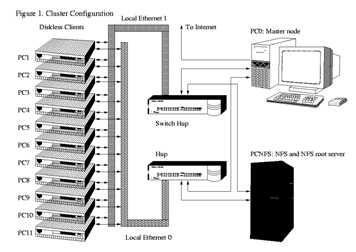
\includegraphics[height=6cm]{gambar/mpii}
\end{figure}

\subsection{Non Klaster}
\emph{Non klaster } adalah komputer yang digunakan dalam proses penyelesaian permasalahan yang ditemui tanpa mengnunakan komputasi paralel dan metode klaster sehingga jika tidak mengunakan super komputer atau komputer yang memiliki spesifikasi yang sesuai dengan syarat yang ditentukan akan memberikan hasil dan waktu proses penyelesaian yang lama bahkan tidak daapat menjalankan program yang ada.


\subsection{Message Pasing Interfaces (MPI)}
MPI \emph{(Message Passing Interface)} adalah spesifikasi API \emph{(Application Programming Interface)} yang memungkinkan terjadinya komunikasi antar komputer pada network, dalam usaha untuk menyelesaikan suatu tugas. Paradigma Message - Passing dengan implementasi MPI memberikan suatu pendekatan yang unik dalam membangun suatu software dalam domain fungsi tertentu, yang dalam hal ini pada lingkungan sistem terdistribusi, sehingga memberikan kemampuan pada produk software yang dibangun diatas middleware tersebut untuk dapat mengeksploitasi kemampuan jaringan komputer dan komputasi secara paralel.


\subsection{Paralel Virtual Imachine (PVM)}
Parallel Virtual Machine \emph{(disingkat PVM)} adalah sebuah perangkat lunak yang digunakan untuk pembuatan jaringan komputer paralel. Perangkat lunak ini didesain sedemikian rupa untuk mengizinkan sebuah jaringan komputer yang heterogen yang terdiri atas mesin yang menjalankan sistem operasi Windows atau Unix agar digunakan sebagai sebuah prosesor paralel tunggal yang terdistribusi. Hal ini bertujuan untuk menyelesaikan beberapa masalah komputasi secara lebih mudah dengan menggunakan kemampuan pemrosesan dan memori dari komputer-komputer yang terjaring tersebut. Perangkat lunak itu sendiri bersifat portabel, dan kode sumbernya pun tersedia secara bebas melalui netlib, yang sekarang telah dikompilasi untuk digunakan oleh beragam jenis komputer, dari mulai laptop hingga superkomputer Cray. 

PVM mengizinkan pengguna untuk menggunakan perangkat keras komputer yang telah ada untuk menyelesaikan problem yang lebih rumit pada harga yang lebih murah. PVM juga digunakan sebagai alat bantu dalam akademisi, khususnya untuk mengajarkanpemrograman paralel \emph{(dalam fakultas ilmu komputer, dan tentu saja digunakan untuk menyelesaikan beberapa masalah praktikal)} .




%-------------------------------------------------------------------------------
\chapter{METODOLOGI PENELITIAN}

\section{Alat dan Bahan}
Dalam penelitian ini mengunakan beberapa alat yang terdiri dari perangkat keras dan perangkat lunak. Adapun rincian dalam penelitian ini sebagai berikut :
\vspace{1cm}

1. PERANGKAT KERAS
\vspace{-0.5cm}
\begin{enumerate}[a.]
\begin{singlespace}
\itemsep0em
\item 1 komputer dengan pengolah pentium 4, 2GHZ, Memory DDRAM 256MB, HDD 40 GB Dan NIC 3 Com 3c905 Boomerang.
\item Kabel UTP Kategori 5 dengan konector RJ45
\item 1 HUB/SWITCH Cisco Catalys seri 2950
\item 1 CDROM untuk Instalasi perangkat lunak
\item 1 Keyboard, monitor dan mouse
\end{singlespace}
\end{enumerate}

2. PERANGKAT LUNAK
\vspace{-0.5cm}
\begin{enumerate}[a.]
\begin{singlespace}
\itemsep0em
\item Sistem operasi RedHat Linux 8.0 dengan kernel 2.4.20 xMOSIX 1.9.0 untuk kernel 2.4.20 
\item MPICH 1.2.5 sebagai perangkat lunak message passing 
\item Compiler gcc versi 3.2 
\item Program ganglia versi 2.5.3 untuk memantau klaster melalui  web browser 
\item Program benchmark HPL versi 1.0 
\item Program  benchmark throughput jaringan netperf versi 2.2 p14
\item Program DFT++ Versi 3.0
\item Library FFTW Versi 2.1.3
\item Library  ATLAS versi 3.4.1 yang menyediakan LAPACK secara lengkap
\end{singlespace}
\end{enumerate}

\section{Metode Pengumpulan Data}
Ada tiga metode pengumpulan data yang penulis gunakan yaitu : 

%\vspace{-0.5}
\begin{enumerate}[1.]
%\begin{singlespace}
\item Metode Observasi Dalam hal ini dilakukan adalah melihat serta mempelajari secara konflik yang ada dilapangan yang erat kaitannya dengan objek yang diteliti. 
\item Metode Studi Pustaka Metode yang dilakukan adalah dengan cara mencari bahan yang mendukung dalam pendefenisian permasalahan melalui buku ,internet yang berkaitan dengan objek permasalahan.
\end{enumerate}

\section{Jadwal Kegiatan}
Penelitian direncanakan akan dilaksanakan selama enam bulan. Rincian rencana jadwal penelitian dicantumkan dalam tabel berikut.

\begin{center}
Tabel 3.1. Jadwal Penelitian.
\end{center}
\vspace{-0.5cm}
\begin{figure}[ht!]
  \centering
    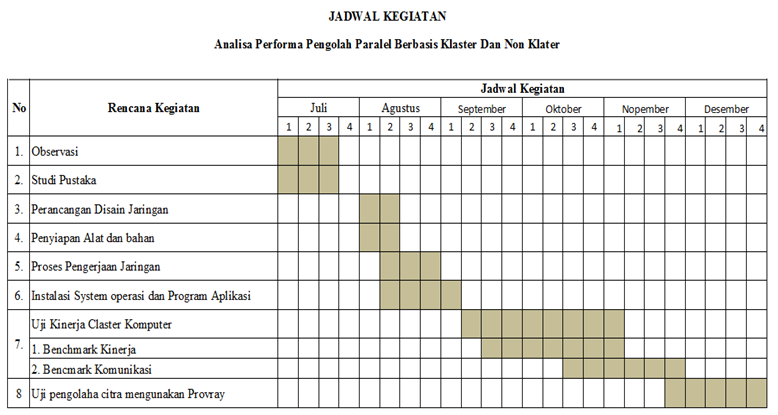
\includegraphics[width=13cm]{gambar/jadwal}
\end{figure}

%-----------------------------------------------------------------
%Disini akhir masukan Bab
%-----------------------------------------------------------------

%-----------------------------------------------------------------
%Disini awal masukan untuk Daftar Pustaka
%-----------------------------------------------------------------
%%\nocite{Abel2010,Guerbas201350}
%%\bibliography{research-plan}
%%\bibliographystyle{plainnat}
\begin{thebibliography}{9}

\bibitem[satu(2013)]{satu01}
Rajkumar Buyya, “High Performance Cluster Computing volume 2”, http://www.cs.mu.oz.au/ raj/cluster/,  Sept. 11 2003

\bibitem[dua(2013)]{dua02}
Neil MacDonald, “Writing Message Passing Parallel Programs with PI”, 
www.epcc.ed.ac.uk/computing/training/document archive/mpicourse/ mpi-course.pdf, Sept. 11 2003 


\bibitem[tiga(2013)]{tiga03}
Parallel Virtual Machine (PVM) version 3, ttp://www.epm.ornl.gov/pvm/pvm home.html, Sept. 11 2003.

\bibitem[empat(2013)]{empat04}
MPICH-A Portable Implementation of MPI, http://www-unix.mcs.anl.gov/mpi/mpich/, Sept. 11 2003


\end{thebibliography}
\addcontentsline{toc}{chapter}{DAFTAR PUSTAKA}
%-----------------------------------------------------------------
%Disini akhir masukan Daftar Pustaka
%-----------------------------------------------------------------

\end{document}